% **************************************************************
% Hi! Edit this file for your presentation!
% **************************************************************

% ==================///==================///==================///
% ==================/// LATEX'S STUFF
% ==================///==================///==================///

\documentclass{beamer}
\usepackage{amsfonts,amsmath,oldgerm}
\usepackage[italian]{babel}
\usepackage[utf8]{inputenc}
\usepackage{bussproofs}\EnableBpAbbreviations
\usepackage{xcolor}

\usetheme{_statale}
\usefonttheme[onlymath]{serif}

\newcommand{\testcolor}[1]{\colorbox{#1}{\textcolor{#1}{test}}~\texttt{#1}}
\newcommand{\hrefcol}[2]{\textcolor{cyan}{\href{#1}{#2}}}
\newcommand{\tto} {\leftrightarrow}
\titlebackground*{assets/background}
\definecolor{darkgreen}{RGB}{0,100,0}

% ==================///==================///==================///
% ==================/// SPLASH PAGE
% ==================///==================///==================///

\title{IMPLEMENTAZIONE IN JAVA DEL METODO DI RISOLUZIONE PER LA LOGICA CLASSICA, ED ESTENSIONE A LOGICHE MODALI}
% \subtitle{Using \LaTeX\ to prepare slides}
\course{Corso di Laurea in Informatica}
\author{Nicolò Iaccarino}
\IDnumber{903870}

% ==================///==================///==================///
% ==================/// START PRESENTATION
% ==================///==================///==================///

\begin{document}
\maketitle

\footlinecolor{maincolor}

% ==================///==================///==================///
% ==================/// BODY'S PRESENTATION
% ==================///==================///==================///

\section{Introduzione}

\begin{frame}{Obiettivi della tesi}
    \begin{itemize}
        \item \textbf{Obiettivo}: implementare in Java il metodo di risoluzione per logiche modali non-normali, partendo dall'implementare il metodo per la logica classica.
        \vspace{10px}
        \item il metodo di risoluzione per la logica classica è già noto, e già implementato.
        \vspace{10px}
        \item il metodo di risoluzione per logiche modali non-normali è descritto in un recente articolo, e mai implementato.
        \vspace{10px}
    \end{itemize}
    
    
\end{frame}

\begin{frame}{Il metodo di risoluzione}
    \begin{itemize}
        \item \textbf{metodo di risoluzione}: sistema di calcolo per inferire la soddisfacibilità di un \emph{insieme di clausole} $S$.
        \vspace{10px}
        \item \textbf{Insieme di clausole}: formula scritta in \emph{Forma normale congiuntiva} (CNF).
        \vspace{10px}
        \item \textbf{Clausola}: insieme di letterali.
    \end{itemize}
    \vspace{20px}

    Vediamo ora il metodo di risoluzione per la logica classica.
\end{frame}


\section{Logica classica}
\begin{frame}{Il metodo di risoluzione per la logica classica}
    \begin{itemize}
        \item Le clausole contengono letterali proposizionali.
        \vspace{10px}
        \item Un insieme $S$ di clausole è \textbf{soddisfacibile} sse esiste interpretazione che soddisfa \textbf{tutte} le clausole in $S$.
        Ad esempio:
        \[S \; = \; \{ \quad \{a, \lnot b\}, \{b, \lnot c\}, \{\lnot a, c\} \quad \}\]
        è un insieme di clausole soddisfacibile con tre clausole.
        \vspace{10px}
        \item Viene utilizzata una sola regola di inferenza: la \textbf{regola di risoluzione} (\emph{Res}). A partire da due premesse $C_1, C_2 \in S$ si genera una risolvente $R$.
    \end{itemize}
\end{frame}

\begin{frame}{Regola di risoluzione}
    \begin{itemize}
        \item Per applicare \emph{Res} è necessario che esista un letterale $L \in C_1$ ed il suo opposto $\overline{L} \in C_2$. Si cancellano $L$ e $\overline{L}$ e si uniscono le due clausole.
        Esempio:
        \[
            \AXC{$\overbrace{\{ a, b \}}^{C_1}$}
            \AXC{$\overbrace{\{\lnot b, c, d \}}^{C_2}$}
            \RightLabel{Res}
            \BIC{$\underbrace{\{ a, c, d \}}_{R}$}
            \DP
        \]
        \item $R$ è la \textbf{risolvente}. Viene aggiunta a $S$ se non è tautologica e non è già presente.
        
    \end{itemize}

    \begin{center}
        \begin{minipage}{0.45\textwidth}
            \begin{itemize}
                \item Lo scopo è trovare la clausola vuota.
            \end{itemize}
            Se la trova $\implies$ S è \textcolor{red}{INSODDISFACIBILE}

            Se non la trova $\implies$ S è \textcolor{darkgreen}{SODDISFACIBILE}
        \end{minipage}
        \hspace{0.05\textwidth}
        \begin{minipage}{0.45\textwidth}
            \small
            \[
                \AXC{$\overbrace{\{ a\}}^{C_1}$}
                \AXC{$\overbrace{\{\lnot a\}}^{C_2}$}
                \RightLabel{Res}
                \BIC{$\underbrace{\{\}}_{R}$}
                \DP
            \]
        \end{minipage}
    \end{center}
\end{frame}

% \section{Clausificazione}

\begin{frame}{Clausificazione di una formula}
    \begin{itemize}
        \item per verificare soddisfacibilità di una formula arbitraria F bisogna prima eseguire la clausificazione.
        \item \textbf{Clausificazione}: conversione di una formula in insieme di clausole equivalente.
        \item per effettuare la clausificazione si applicano le regole di inferenza:
        \begin{itemize}
            \item \textbf{Eliminazione della doppia implicazione}
            \item \textbf{Eliminazione dell'implicazione}
            \item \textbf{Proprietà distributiva di $\lor$ su $\land$}
            \item \textbf{Doppia negazione}
            \item \textbf{Leggi di De Morgan}
        \end{itemize}
        % \item Le regole vengono applicate ricorsivamente sulle sottoformule.
        \item Esempio: $\quad F = (a \lor b) \to c$ \\diventa: $\quad S = \{ \; \{\lnot a, c\}, \{\lnot b, c\} \; \}$
    \end{itemize}
    
\end{frame}

\section{Logiche modali non-normali}
\begin{frame}{Metodo di risoluzione per le logiche modali non-normali}
    \begin{itemize}
        \item I letterali possono essere \emph{proposizionali} o \emph{modali}. 
        \item $\Box p$ e $\lnot \Box p$ sono modali.
        \item Le clausole sono di due tipi:
        \begin{itemize}
            \item \textbf{Clausola locale (classica)}: \[ l_1 \lor l_2 \lor \ldots \lor l_n \]
            \item \textbf{Clausola \textcolor{red}{globale}}: \[ G(l_1 \lor l_2 \lor \ldots \lor l_n) \]
        \end{itemize}
        dove $l_i$ è un letterale.
        \item Consideriamo la logica modale non-normale minimale \textbf{E}. Per questa logica il metodo di risoluzione applica le regole $RES_E$. 
    \end{itemize}

\end{frame}

\begin{frame}{Regole di risoluzione $RES_E$}
    \begin{itemize}
        \item Le regole $RES_E$ sono:
        \begin{figure}
            \centering
            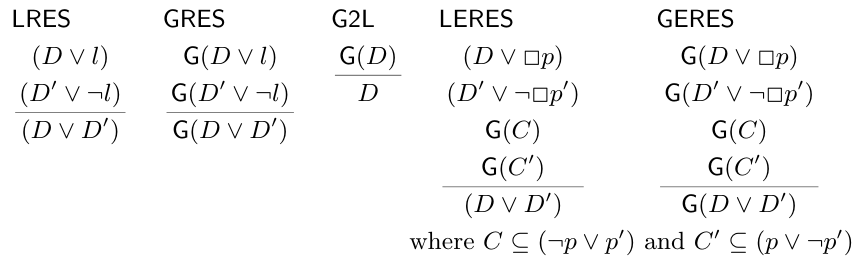
\includegraphics[width=0.7\textwidth, height=0.5\textheight]{assets/res_E.png}
        \end{figure} 
        \item Dove $C$ e $D$ sono clausole, $l$ è un letterale, e $p$ è una variabile proposizionale.
        \item Come nella logica classica, lo scopo è trovare la clausola vuota.
    \end{itemize}
\end{frame}

\begin{frame}{Clausificazione di formule modali}
    \begin{itemize}
        % \item Le formule modali usano il connettivo \emph{box} ($\Box$).
        \item Sia $\phi$ una formula. Occorre introdurre nuove variabili proposizionali per rappresentare le sottoformule di $\phi$. Questo viene fatto con la funzione $\eta$.
        \[
            \eta: \quad subf(\phi) \mapsto V \setminus V(\phi)
        \]
        \item Per la clausificazione di $\phi$ si usa la funzione di riduzione \textbf{R}.
        \item L'insieme di clausole equivalente a $\phi$ è: $\{ \eta(\phi) \} \cup R(G(\eta(\phi) \tto \phi))$.
        \item \textbf{R} è così definita:
        \[
            \begin{aligned}
            R(G(t \tto p)) &= \{ G(\lnot t \lor p), G(t \lor \lnot p) \} \\
            R(G(t \tto \lnot \psi)) &= \{ G(\lnot t \lor \lnot \eta(\psi)), G(t \lor \eta(\psi)) \} \cup R(G(\eta(\psi) \tto \psi)) \\
            R(G(t \tto \psi \lor \psi')) &= \{ G(\lnot t \lor \eta(\psi) \lor \eta(\psi')), G(t \lor \lnot \eta(\psi)), G(t \lor \lnot \eta(\psi')) \} \\
            & \quad \cup R(G(\eta(\psi) \tto \psi)) \cup R(G(\eta(\psi') \tto \psi')) \\
            R(G(t \tto \Box \psi)) &= \{ G(\lnot t \lor \Box \eta(\psi)), G(t \lor \lnot \Box \eta(\psi)) \} \cup R(G(\eta(\psi) \tto \psi))
            \end{aligned}
        \]
    \end{itemize}
\end{frame}

\section{Utilizzo pratico del metodo di risoluzione}

\begin{frame}{Verificare la validità di una formula}
    \begin{itemize}
        \item L'utilizzo pratico implementato è la verifica della \textbf{validità} di una formula $F$.
        \vspace{5px}
        \begin{center}
            F è \textbf{valida} $\iff$ $\lnot F$ è \textbf{insoddisfacibile}
        \end{center}
        \vspace{5px}
        \item Per verificare se $F$ è valida:
        \begin{itemize}
            \item si nega $F$, ottenendo $\lnot F$.
            \item si effettua la clausificazione su $\lnot F$ e si ottiene l'insieme di clausole equivalente $S$.
            \item si applica il metodo di risoluzione su $S$.
        \end{itemize}
        \item Se $S$ è insoddisfacibile $\implies$ $F$ è \textcolor{darkgreen}{VALIDA}.
        \item Se $S$ è soddisfacibile $\implies$ $F$ è \textcolor{red}{NON VALIDA}.
    \end{itemize}
\end{frame}

\begin{frame}{Esempio (su logica classica)}
    \begin{itemize}
        \item Consideriamo la seguente formula $F$:
        \[
            F \; = \; (a \land (a \to b)) \to b
        \]
        \item applicando la clausificazione su $\lnot F$ si ottiene il seguente insieme di clausole $S$:
        \[
            S \; = \; \{\quad \{a\}, \{\lnot a, b\}, \{\lnot b\} \quad\}
        \]
        \item eseguendo il metodo di risoluzione si trova la clausola vuota in due passaggi:
        
    \end{itemize}
    \begin{center}
        \begin{minipage}{0.45\textwidth}
            \[
                \AXC{$\overbrace{\{ a\}}^{C_1}$}
                \AXC{$\overbrace{\{\lnot a, b\}}^{C_2}$}
                \RightLabel{Res}
                \BIC{$\underbrace{\{b\}}_{R}$}
                \DP
            \]
        \end{minipage}
        \hspace{0.05\textwidth}
        \begin{minipage}{0.45\textwidth}
            \[
                \AXC{$\overbrace{\{ b\}}^{C_1}$}
                \AXC{$\overbrace{\{\lnot b\}}^{C_2}$}
                \RightLabel{Res}
                \BIC{$\underbrace{\{\}}_{R}$}
                \DP
            \]
        \end{minipage}
    \end{center}

    \begin{itemize}
        \item $\lnot F$ è insoddisfacibile, questo dimostra che $F$ è valida.
    \end{itemize}
    
\end{frame}

\begin{frame}{Tecnologie utilizzate}
    \begin{itemize}
        \item \textbf{Visual Studio Code}: ambiente utilizzato per programmare in Java.
        \vspace{10px}
        \item \textbf{ANTLR4}: per effettuare parsing di formule.
        \vspace{10px}
        \item \textbf{Junit}: per eseguire il testing del metodo di risoluzione.
    \end{itemize}
\end{frame}

% ==================///==================///==================///
% ==================/// END PRESENTATION
% ==================///==================///==================///

\backmatter

\end{document}